\documentclass[Naxsi]{subfiles}
\begin{document}
\section{Naxsi}
\label{sec:Naxsi}
Naxsi is written to be a fast, light and scalable \ac{WAF} for the Nginx web server. Naxsi stands for \textit{Nginx Anti Xss \& Sql Injection} and it has a positive approach for web traffic inspection by using a whitelisting method. This means that traffic is blocked by default, and "good" traffic must explicitly be allowed. Naxsi uses two different files, which contain the rules. First, at the server level configuration. Second, at the HTTP location level configuration. The first one is called the core rules, and it contains regular expressions for most of the characters that are usually involved in an attack. Upon match, it will increase the score of the request. The location level configuration has site specific rules and, thus allows for multiple virtual hosts for having different whitelists and thresholds for the score of a request. Naxsi will deny the request, when the threshold is exceeded. The core level configuration can be referred to as blacklist. Furthermore it is more or less a fixed list and, according to the Naxsi website~\footnote{\url{https://code.google.com/p/naxsi/wiki/HowDoesItWork}}, it is not expected to evolve rapidly. On the other hand, the location level configuration is a site specific configuration, and thus needs to be created. Creating the rules is done by putting Naxsi in learning mode. When Naxsi is in learning mode, requests are not blocked, but are rather seen as valid traffic and used for creating the whitelist rule set.

\subsection{Request flow}
When Naxsi is in production mode, it actively gives each request a score. Depending on the location level configuration rule set, the request may be allowed or dropped. Figure~\ref{fig:naxsi_flow} shows how logically each request is processed by Naxsi. First, the request is checked for "dangerous" symbols and SQL keywords. Second, the request is checked by the location level rules. Location level rules may overrule the core rules. Lastly, the request score is checked against the rule set. Depending on the score, the request is either blocked, which means that the request gets forwarded to the \textit{DeniedURL}, or the request is further processed. The \textit{DeniedUrl} is set in the location level configuration whitelist file. This allows the administrator to specify what should be returned to the client when a bad request is sent.

\begin{figure}[h]
\caption{Naxsi request flow}
\centering
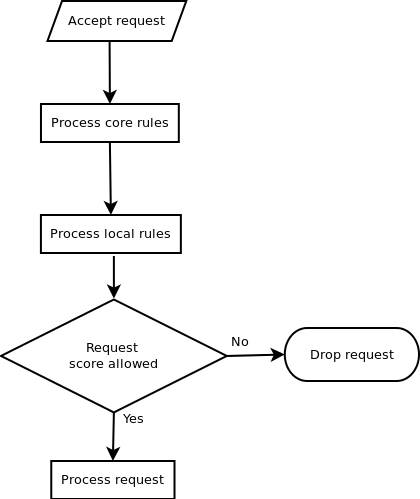
\includegraphics[width=0.5\textwidth] {images/naxsi_flow.png}
\label{fig:naxsi_flow}
\end{figure}

\subsection{Whitelist processing}
\label{sec:naxsi_whitelist}
As already mentioned, Naxsi does have a short blacklist. However, the usage of whitelists is more extensive, as each location level configuration contains a separate set per virtual host. At startup Naxsi generates up to four zone hash tables from the location level whitelist rules in memory, as can be seen in figure~\ref{fig:hashtables}. The respective zones are:
\begin{itemize}
	\item ARGS (GET arguments)
	\item URL (the full URI)
	\item BODY (POST arguments)
	\item HEADER (HTTP headers)
\end{itemize}

\begin{figure}[h]
\caption{Creating hash tables from location level rules}
\centering
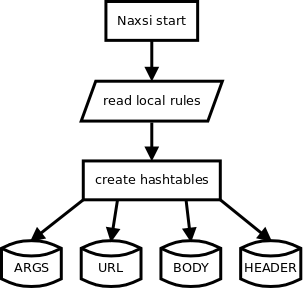
\includegraphics[width=0.5\textwidth] {images/hashtables.png}
\label{fig:hashtables}
\end{figure}

As visualized in figure~\ref{fig:whitelist_processing}, once an HTTP request is accepted, it is parsed and split up into four streams corresponding to the zones: ARGS, URL, BODY, HEADERS. Each stream, that may consist of more parameters, is iterated independently, but in the same manner. Each parameter is checked for suspicious patterns, by consulting the core rules. Furthermore, a lookup in the respective zone hash table is done, as to determine whether this specific match is whitelisted. If it is not whitelisted, the score that is attached to the matching core rule is applied. When all streams are processed, then eventually it is determined if the total score for (SQL, RFI, TRAVERSAL, XSS) is below the threshold. If it is, the request is forwarded. If not, it is denied. 

\begin{figure}[H]
\caption{Naxsi whitelist processing}
\centering
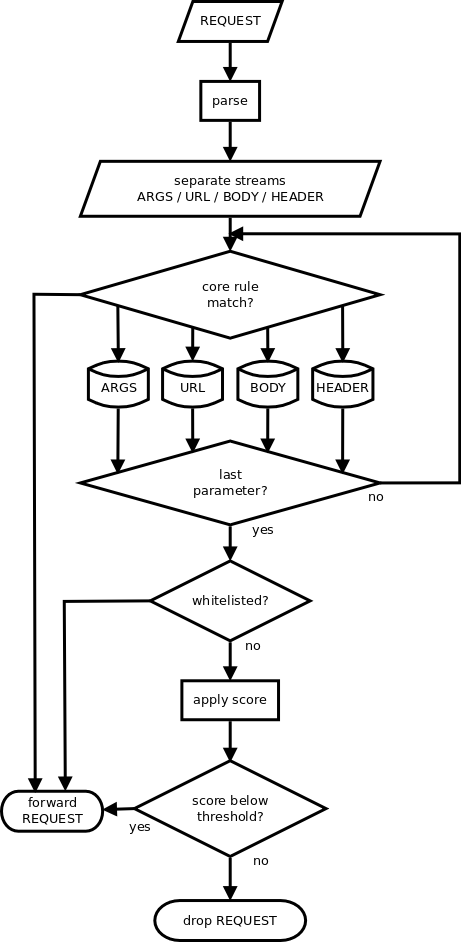
\includegraphics[width=0.4\textwidth] {images/whitelist_processing.png}
\label{fig:whitelist_processing}
\end{figure}

This approach shows that matching is done very efficient. Creating hash tables from the whitelists in memory, accelerates the process of lookups. Furthermore, through splitting up the REQUEST data in the same manner as the hash tables, the processing of parameters is handled separately. This allows for lookups to be only done, when there is a need for it. If, for example, a request contains a few URL parameters, but only one of them is 'suspicious', each parameter is matched against the (short list of) core rules, but only the suspicious one is further analysed.

\end{document}
